\chapter{Preliminaries}
\label{chap:preliminaries}

\tamara{I'm unsure about the overall structure of this chapter: it's a little dry as it stands right now. Do we really want formal definition environments? Do we need some more discussion of the concepts outside of the formal definitions? Do we need citations for the more exotic and/or controversial definitions (as for rectilinear dual)?}

\tamara{I would like to keep this chapter as a \quoted{refresher} of things one could reasonably already know, and define my own things such as \emph{polygonal dual} and \emph{approximate proportional contact representations} in the following chapters once I need them. Is this ok?}

\tamara{Do we need more figures in this chapter?}

% https://math.stackexchange.com/questions/566565/are-if-and-iff-interchangeable-in-definitions

\paragraph{Notation}

When dealing with sets, we use the operator $+$ in place of $\cup$ when we want to emphasize that the operands are disjoint. Similarly, we use the operator $-$ in place of $\setminus$ to stress that the right operand is a subset of the left operand. We sometimes use set elements where sets would be mathematically correct, \eg{} $\{1,2\} + 3 = \{1,2,3\}$. This is to be interpreted as the element being wrapped in a set implicitly.


\paragraph{Graphs}

\begin{definition}
	A \emph{(simple, undirected) graph} $G$ is a tuple $G = (V, E)$ of \emph{vertices} $V$ and \emph{edges} $E \subseteq \left\{\{u,v\} \vert (u,v) \in V^2 \right\}$.
	For an arbitrary graph $H$ we sometimes denote its vertices by $V(H)$ and its edges by $E(H)$.
	Graphs can be weighted, assigning real-values weights to its vertices and/or edges. We differentiate between vertex-weighted graphs that provide a weight function $w_v \colon V \to \mathbb{R}$ and edge-weighted graphs that provide a weight function $w_e \colon E \to \mathbb{R}$.
\end{definition}

When graphs are weighted, we typically include the weight functions in the graph tuple, \eg{} $G_w = (V,E,w_v)$. Of course, graphs can be both vertex- and edge-weighted.

\begin{definition}
	Given a graph $G = (V, E)$, two vertices $u, v \in V, u \neq v$ are said to be \emph{adjacent} if there's an edge connecting $u$ to $v$, \ie{} $\{u, v\} \in E$.
	Adjacent vertices are also called \emph{neighbors}.
	A vertex' \emph{degree} is its number of neighbors.
	An edge $e = \{u, v\} \in E$ is said to be \emph{incident} to its \emph{endpoints} $u$ and $v$.
	Two edges $\{u,v\}, \{v,w\} \in E$ are also said to be \emph{incident} if they share exactly one endpoint $v$.
\end{definition}

\begin{definition}
	A \emph{path} $p$ is a nonempty sequence of edges that connects a sequence of distinct vertices $(v_1, \dots, v_n)$, \ie{} $p = (\{v_1, v_2\}, \dots, \{v_{n-1},v_n\}) \land \forall i \neq j \colon v_i \neq v_j$.
	The first and last vertices $v_1, v_n$ of a path are called its \emph{endpoints}.
	A path $p$'s \emph{length} $l(p)$ is the number of edges in the path.
\end{definition}

\begin{definition}
	A graph $G = (V, E)$ is \emph{connected} if there exists a path between any pair of vertices in the graph.
	$G$ is said to be \emph{$k$-(vertex)-connected} if one needs to remove $k$ or more vertices and their incident edges to disconnect $G$.
\end{definition}



\paragraph{Graph Operations}

\begin{definition}
	Given a graph $G = (V, E)$, one can \emph{subdivide} an edge $e \coloneqq \{u,v\} \in E$ by removing the edge $e$ and inserting a new vertex $w$ with edges to both $u$ and $v$. This produces a graph $G^\prime = (V^\prime, E^\prime)$ with $V^\prime = V + w$ and $E^\prime = E - \{u,v\} + \{u,w\} + \{w,v\}$.
	A graph $H$ is said to be a \emph{subdivision} of $G$ if $H$ can be obtained from $G$ by repeatedly subdividing edges.
	$H$ is a \emph{1-subdivision} of $G$ if it can be obtained from $G$ by subdividing every edge exactly once.
\end{definition}

% https://en.wikipedia.org/wiki/Homeomorphism_(graph_theory)#Subdivision_and_smoothing
\begin{definition}
	Similarly, a vertex $v$ of degree 2 can be \emph{smoothed}, replacing it and its incident edges with a new edge $\{u,w\}$ between its original neighbors.
\end{definition}

\begin{definition}
	One can also \emph{contact} an edge $\{u,v\}$, deleting it and \quoted{merging} its endpoints.
	This removes the edges $E_- \coloneqq \{ \{x,y\} \in E \vert u \in \{x,y\} \lor v \in \{x,y\} \}$ and creates new edges $E_+ \coloneqq \{ \{uv,x\} \vert \{u,x\} \in E \lor \{v,x\} \in E \}$, producing a new graph $G^\prime = (V^\prime, E^\prime)$ with $V^\prime = V - u - v + uv$ and $E^\prime = E - E_- + E_+$.
%	Contracting an edge $\{u,v\}$ is only permitted if $u$ and $v$ don't have any neighbors in common.
% Path contraction? https://en.wikipedia.org/wiki/Edge_contraction#Path_contraction
\end{definition}



\paragraph{Graph Drawings}

% http://www.planarity.org/Klein_elementary_graph_theory.pdf uses "geometric embedding"
\begin{definition}
	A \emph{drawing} or \emph{topological embedding} of a graph $G = (V, E)$ maps its vertices to distinct points in the plane and its edges to continuous curves between its endpoints in the plane.
	The graph $G$ is called \emph{planar} if it permits a drawing in which its edges don't self-intersect and don't cross other edges, \ie{} the edges only intersect in their endpoints.
	Such a drawing is called a \emph{planar embedding} of $G$. If all edges of $G$ are line segments, we also call it a \emph{planar straight-line embedding}.
	We also use the term \emph{plane graph} to refer to planar graph in combination with a concrete planar embedding.
\end{definition}

\begin{definition}
	A planar embedding divides the plane into mutually disjoint regions called \emph{faces}. We denote the set of faces of a plane graph $G$ by $F(G)$ and use the word face to mean the region in the plane and the set of edges that bound said region interchangeably.
	All faces but one, the \emph{internal faces}, are bounded; the unbounded face is called the \emph{outer face}.
	Two faces are said to be \emph{incident} if they share an edge.
	Similarly, an edge is said to be \emph{incident} to a face if the edge is part of the face's boundary. Edges are always incident to one or two faces.
	A plane graph $G$ can be \emph{face-weighted} if there's a weight function $w_f \colon F_\text{int}(G) \to \mathbb{R}$ assigning real numbers to its internal faces $F_\text{int}(G)$.
\end{definition}

\begin{definition}
	A planar graph $G$ is said to be \emph{triangulated} if adding any edge to $G$ would result in a nonplanar graph. This is the case if all faces are triangles.
	Similarly, a plane graph $G$ is said to be \emph{internally triangulated} if all internal faces are triangles.
\end{definition}

\begin{definition}
	Given a plane graph $G$, its topological embedding defines the cyclic order of the edges incident to a vertex $v$ for all its vertices. The cyclic orders of all vertices of the graph together are called a \emph{combinatorial embedding} of the planar graph $G$.
\end{definition}

Combinatorial embeddings uniquely determine the faces (which edges bound them, not their geometry) any drawing with same combinatorial embedding would have.

\begin{definition}
	A \emph{multigraph} is a graph that, as opposed to a simple graph, is can have multiple edges between a pair of vertices as well as so-called loops, \ie{} edges connecting a vertex to itself.
	The \emph{dual graph} of a plane graph $G$ is a plane pseudograph that has a vertex for every face of $G$ and edges connecting the vertices corresponding to the incident faces of each edge in the graph $G$. The dual graph is embedded in such a way that the dual edges cross their primal edges, but don't cross each other. The dual graph of a plane graph $G$, often abbreviated as just \emph{dual}, is denoted as $G^*$.
	The \emph{weak dual graph} $G^-$ of a plane graph is its dual without the vertex corresponding to the $G$'s outer face\cite{fleischner1974}.
\end{definition}

\begin{figure}[H]
	\centering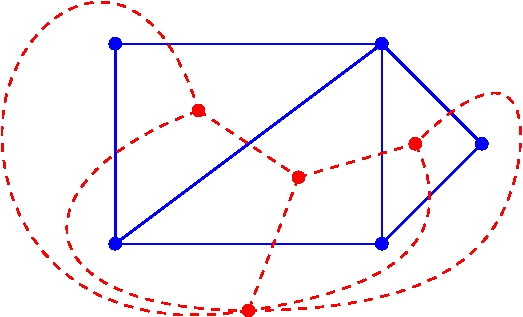
\includegraphics[height=130px]{Resources/Preliminaries-Dual.pdf}
	\caption{A plane graph $G$ (in blue) and its dual $G^*$ (in red).}
	\label{fig:preliminaries-dual}
\end{figure}

An example for a plane graph and its dual is illustrated in \cref{fig:preliminaries-dual}. Forming the dual of a plane graph essentially turns vertices into faces and vice versa and \quoted{flips} the edges of the plane graph as illustrated in \cref{fig:preliminaries-dual}. Note that no matter how the dual graph is embedded (topologically), its combinatorial embedding is uniquely determined by the original plane graph. When forming the dual of the dual of a plane graph, we get back the original plane graph, \ie{} $(G^*)^* = G$. Since combinatorial embeddings uniquely determine the faces, we can also form the dual directly from a combinatorial embedding.

% TODO: Do we even need weak dual, augmented dual?



\paragraph{Contact Representations}

\begin{definition}
	A planar graph $G$ can be represented as a so-called \emph{contact graph}. In such a representation, the vertices are represented by pairwise internally disjoint regions in the plane and edges are implicitly defined between vertices whose regions touch \cite{alam2013linear}.
	Such an arrangement of regions is called a \emph{contact representation} of $G$. If all regions are simple polygons, it is also called a \emph{polygonal contact representation}.
	A contact representation can be \emph{weighted}, assigning a real weight to all of its faces, and is said to \emph{proportional} if the regions' areas are proportional to said weights \cite{alam2013linear}.
	A contact representation is said to be \emph{hole-free} if it contains no area that isn't part of any of the regions \cite{alam2013linear}.
	Given a plane graph $G$, a contact representation of $G$ with axis-aligned rectilinear polygons is called a \emph{rectilinear dual} of $G$ \cite{alam2013computing}.
\end{definition}

\begin{figure}[H]
	\centering
	\subfigure[]{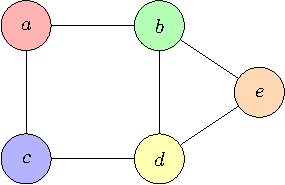
\includegraphics[height=90px]{Resources/Preliminaries-RectilinearDual-Primal.pdf}}
	\quad
	\subfigure[]{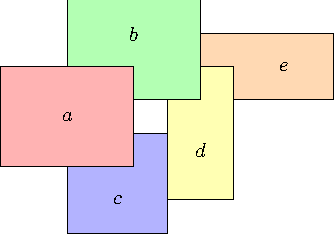
\includegraphics[height=90px]{Resources/Preliminaries-RectilinearDual-Polygons.pdf}}
	\quad
	\subfigure[]{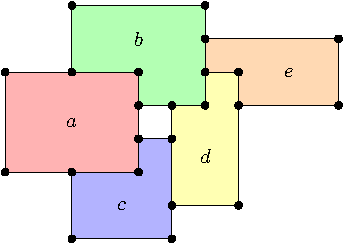
\includegraphics[height=90px]{Resources/Preliminaries-RectilinearDual-Dual.pdf}}
	\caption{A plane graph $G$ (a) and a possible rectilinear dual of $G$ with a hole, as a plain arrangement of polygons (b), and construed as yet another plane graph (c).}
	\label{fig:preliminaries-rectilinear-dual}
\end{figure}

Note that the name \quoted{dual} is fitting here because vertices of the original graph turn into faces, or regions of the rectilinear dual. In fact, we can regard the rectilinear dual as a plane graph itself: the polygons' corners are vertices, connected by edges as determined by the polygons' sides. Also note that one can interpret the rectilinear dual as a plane graph itself, as illustrated in \cref{fig:preliminaries-rectilinear-dual}. We use the term rectilinear dual to refer to the the actual arrangement of rectilinear polygons and the induced plane graph interchangeably.

In the remainder of this thesis, we assume contact representations to be hole-free unless otherwise noted.



\paragraph{Area Universality}

\begin{definition}
	A plane graph $G$ with internal faces $F_\text{int}$ is \emph{area universal} if, for every area assignment of its internal faces $A \colon F_\text{int} \to \mathbb{R}_+$, there exists a planar straight-line drawing of $G$ with the same combinatorial embedding such that all internal faces $f_\text{int}$ have the area $A(f_\text{int})$ as prescribed by $A$.
\end{definition}

Recall that Thomassen \cite{thomassen1992plane} showed that all (planar embeddings of) cubic graphs, \ie{} graphs in which all vertices have degree 3, are area-universal, and that Kleist \cite{kleist2019planar} showed that all plane 1-subdivisions of planar graphs are area-universal, too.
